\section{Model Introduction and Variables}

In this section, we introduce new variables derived from the Fama-French 5-Factor Model and Federal Reserve Economic Data 
(FRED). 
The Fama-French model was developed to improve the evaluation of stock returns.
 It includes:
\begin{enumerate}
    \item \textbf{eMKT:} The excess market returns.
    \item \textbf{Mkt-Rf:} The difference between the market returns of a portfolio (comprising stocks from NYSE, AMEX, or
    NASDAQ) and the risk-free interest rate (one-month Treasury bill).
    \item \textbf{SMB (Small Minus Big):} A factor that captures the size effect by considering the difference in returns
    between small and large-cap stocks.
    \item \textbf{HML (High Minus Low):} Reflecting the value effect, it measures the difference in returns between high and
    low book-to-market value stocks.
    \item \textbf{RMW (Robust Minus Weak):} A profitability factor comparing returns of companies with robust and weak 
    profitability.
    \item \textbf{CMA (Conservative Minus Aggressive):} A factor that considers investment policies, contrasting companies 
    with conservative versus aggressive investment approaches.
\end{enumerate}

To account for the macroeconomic impact on our sector, we used four additional variables:

\begin{enumerate}[resume*]
    % maybe add achronym?
    \item \textbf{CPI (Consumer Price Index):} Representing inflation, we calculated its logarithmic changes to reflect the inflation rate.
    \item \textbf{Oil Prices:} Capturing variations in energy costs.
    \item \textbf{US Industrial Production Index:} Transformed logarithmically to examine coherence with growth rate of the
    industrial sector.
    \item \textbf{Producer Price Index (PPI) for Chemical Manufacturing:} Evaluating how sector-specific costs impact returns.
\end{enumerate}

We included these macroeconomic indicators because they potentially influence costs and returns for companies in our sector.

\section{Model Building and Refinement}

Initially, we estimated a regression model using all variables.
Next, we iteratively removed insignificant variables using the GETS (General-to-Specific) modeling strategy,
which simplifies models while retaining predictive power, the specifics of this process can be found in
Appendix~\ref{appendix:GETS}.
The complete model is presented in Figure~\ref{fig:7_1}.

\begin{figure}[h!]
    \centering
    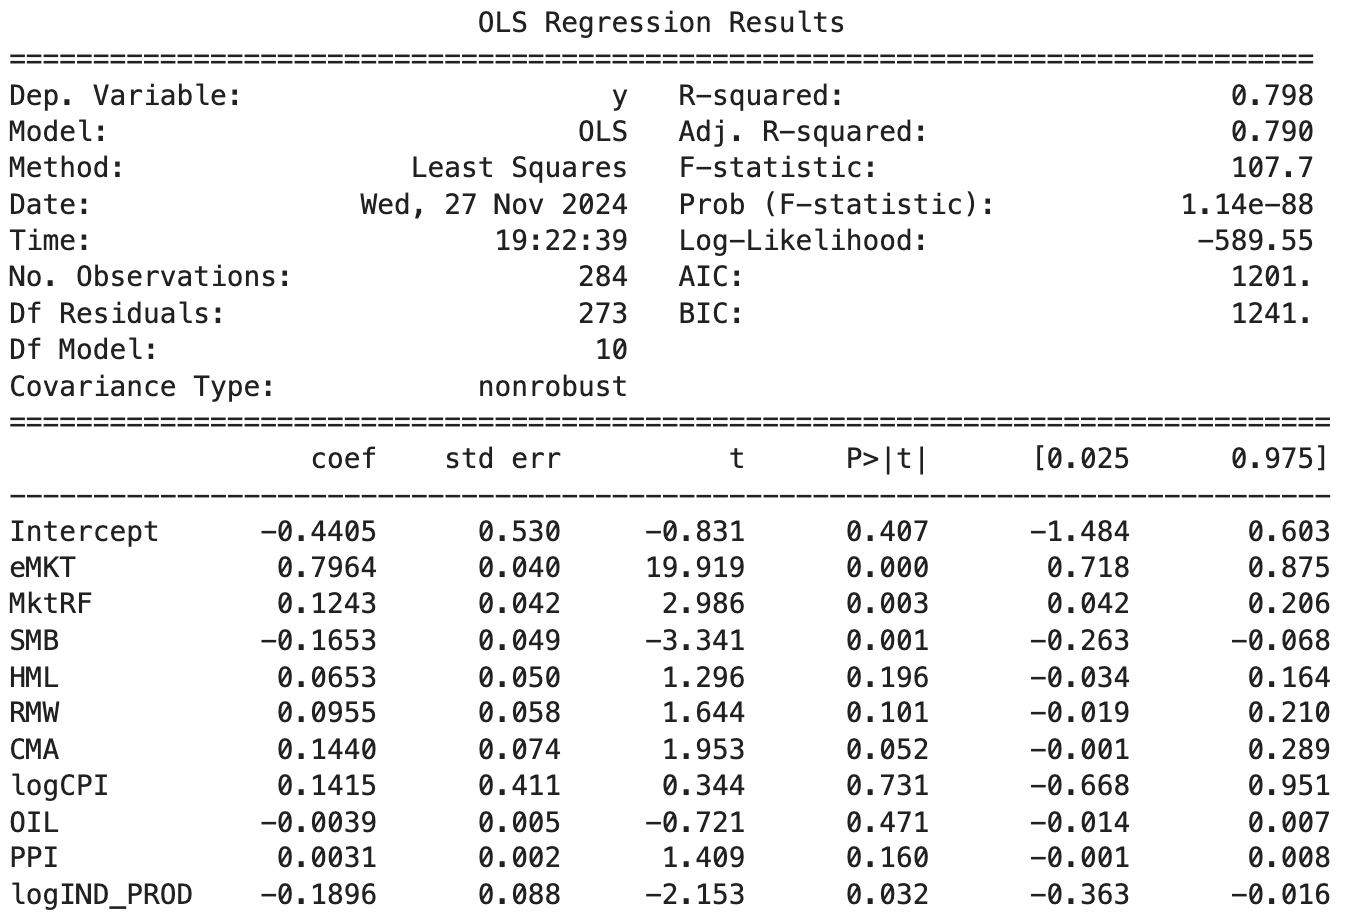
\includegraphics[width=0.8\textwidth]{images/7_1.png}
    \caption{Regression Summary for model complete of all variables.}\label{fig:7_1}
\end{figure}

We can clearly see that many betas are not significant, so it is better if we eliminate and rerun the
model with only the significant ones.
The restricted model includes eMKT, Mkt$\-$Rf, SMB, HML, and IND$\_$PROD.
While the alpha was insignificant, it was retained for comparison purposes. 
For all the following analysis, we will use this model as a benchmark (see Figure~\ref{fig:7_2}).

\begin{figure}[h!]
    \centering
    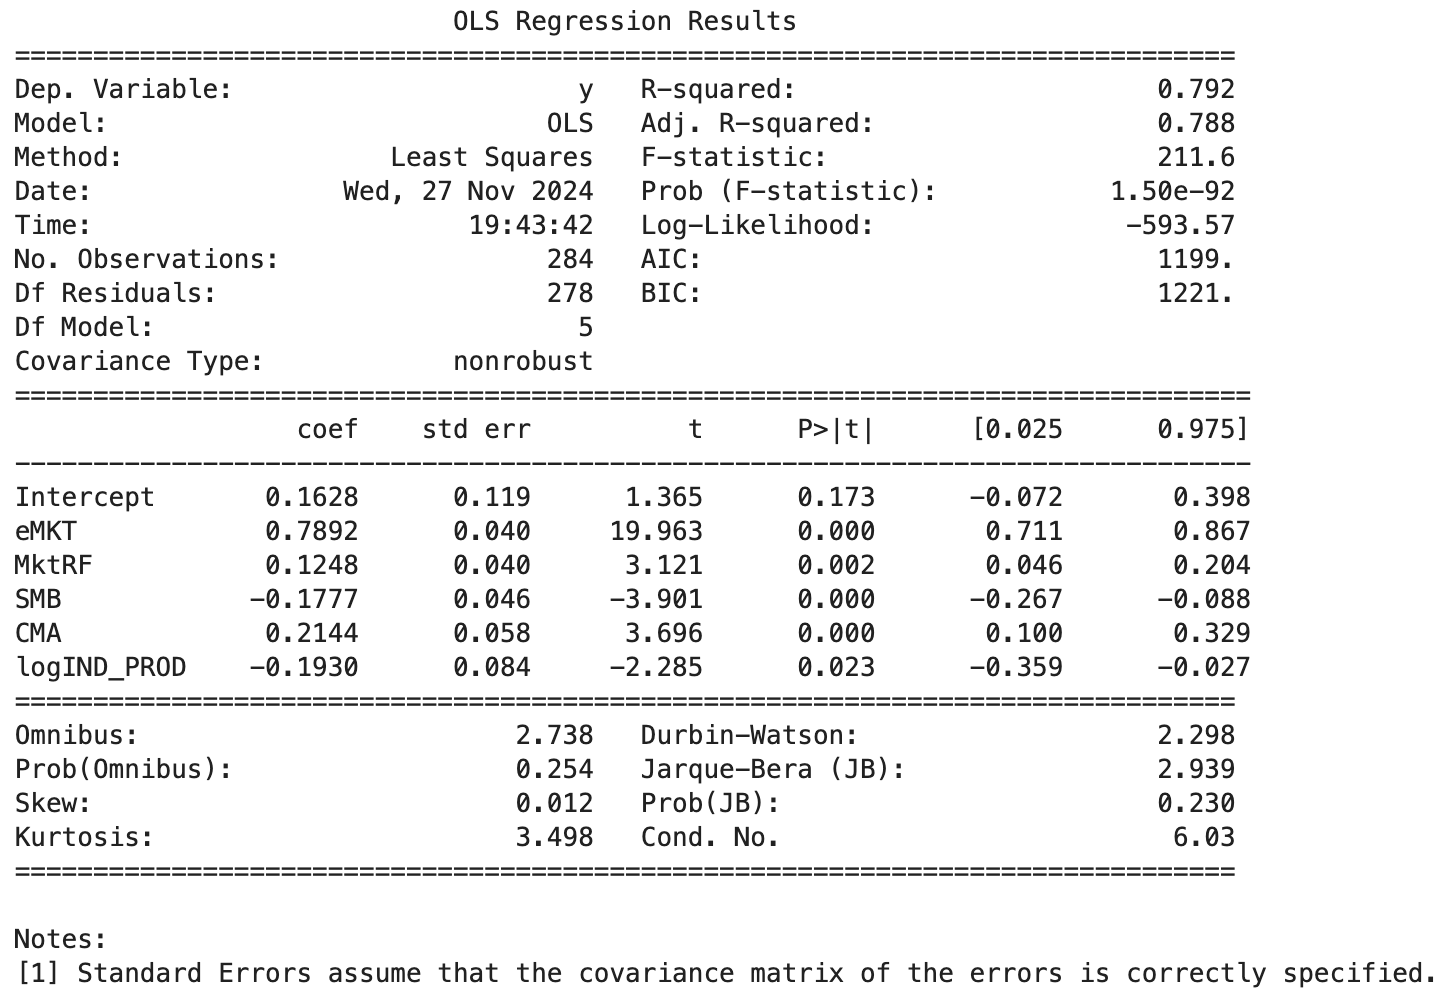
\includegraphics[width=0.8\textwidth]{images/7_2.png}
    \caption{Regression summary for restricted model.}\label{fig:7_2}
\end{figure}

\textbf{Comparison Between Complete and Restricted Models:} The adjusted $R^2$ decreased minimally from 0.790 to 0.788, confirming that the simpler 
model retained explanatory power. 
Moreover, the test on the difference of the residuals between the restricted and the unrestricted model gives a p-value 
equal to 0.1695, so we can agree that the difference in prediction power is not statistically significant.

\textbf{Correlation between variables:} Analyzing the multicollinearity, we observed a high correlation between eMKT and 
Mkt-rf, as shown in Figure~\ref{fig:correlation}. 

\begin{figure}[h!]
    \centering
    \includegraphics[width=0.8\textwidth]{images/correlation.jpeg}
    \caption{Heatmap showing correlation between explanatory variables.}\label{fig:correlation}
\end{figure}

To investigate the impact, we excluded MktRF from the model to assess whether the standard error of eMKT would change
significantly.
After running the adjusted model (Figure~\ref{fig:7_3}), we observed that the standard error decreased, from 0.040 to 0.028.
Despite this drop, we decided to keep MktRF in the model due to its low Variance Inflation Factor (VIF) of 2.618.
This is well below the common threshold of 5, which is typically used to flag potential collinearity issues.
We then examine the correlations among the remaining variables and found no coefficients suggesting the need for further
adjustments or checks.

\begin{figure}[h!]
    \centering
    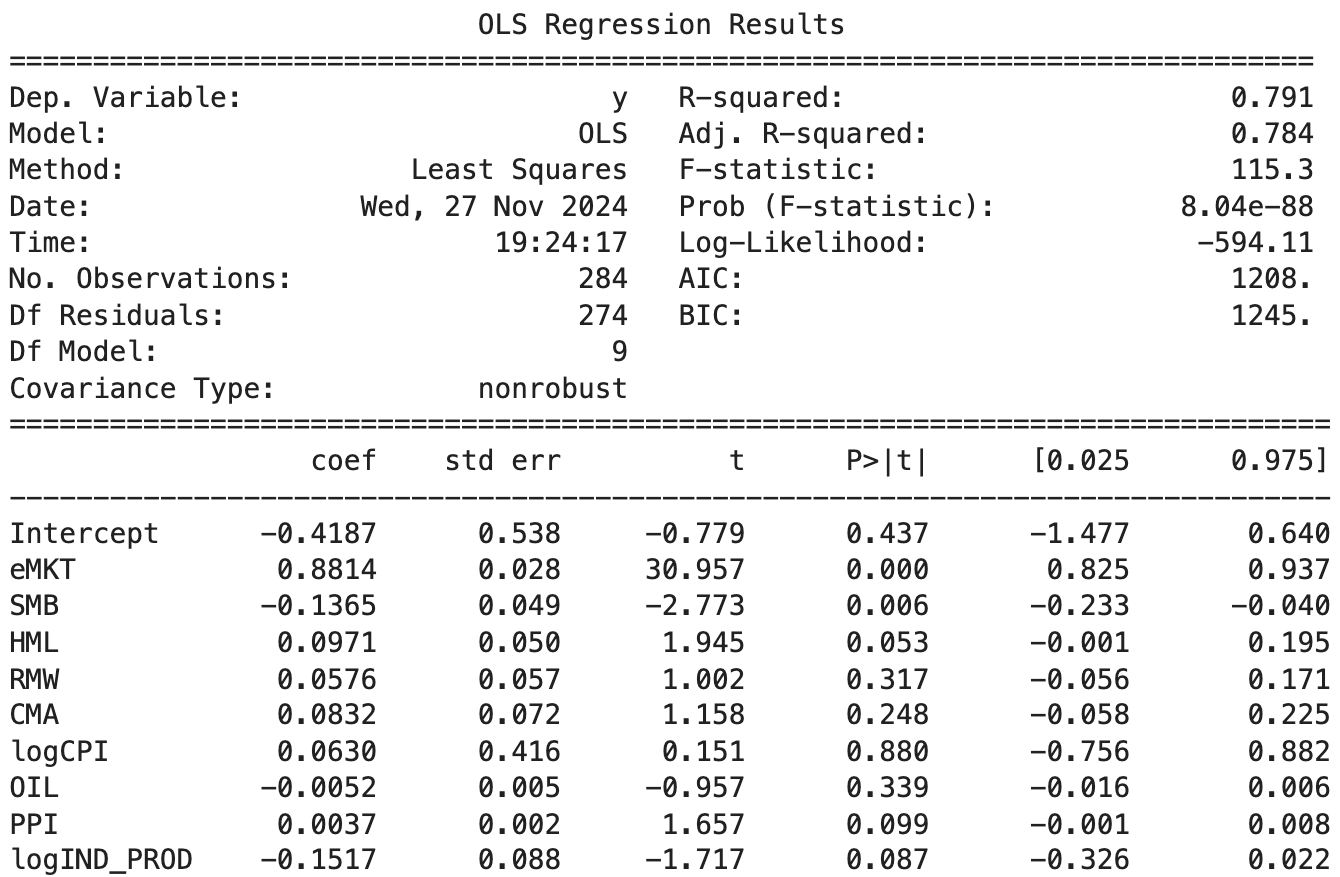
\includegraphics[width=0.8\textwidth]{images/7_3.png}
    \caption{Regression summary for adjusted model.}\label{fig:7_3}
\end{figure}

\subsection{Comparative Analysis}

We estimated the CAPM using the ePortfolio as the dependent variable and eMKT as the independent variable
(Figure~\ref{fig:7_4}).
This model had an adjusted $R^2$ of 0.766, lower than the multivariate model ($R^2$ = 0.788).

\begin{figure}[h!]
    \centering
    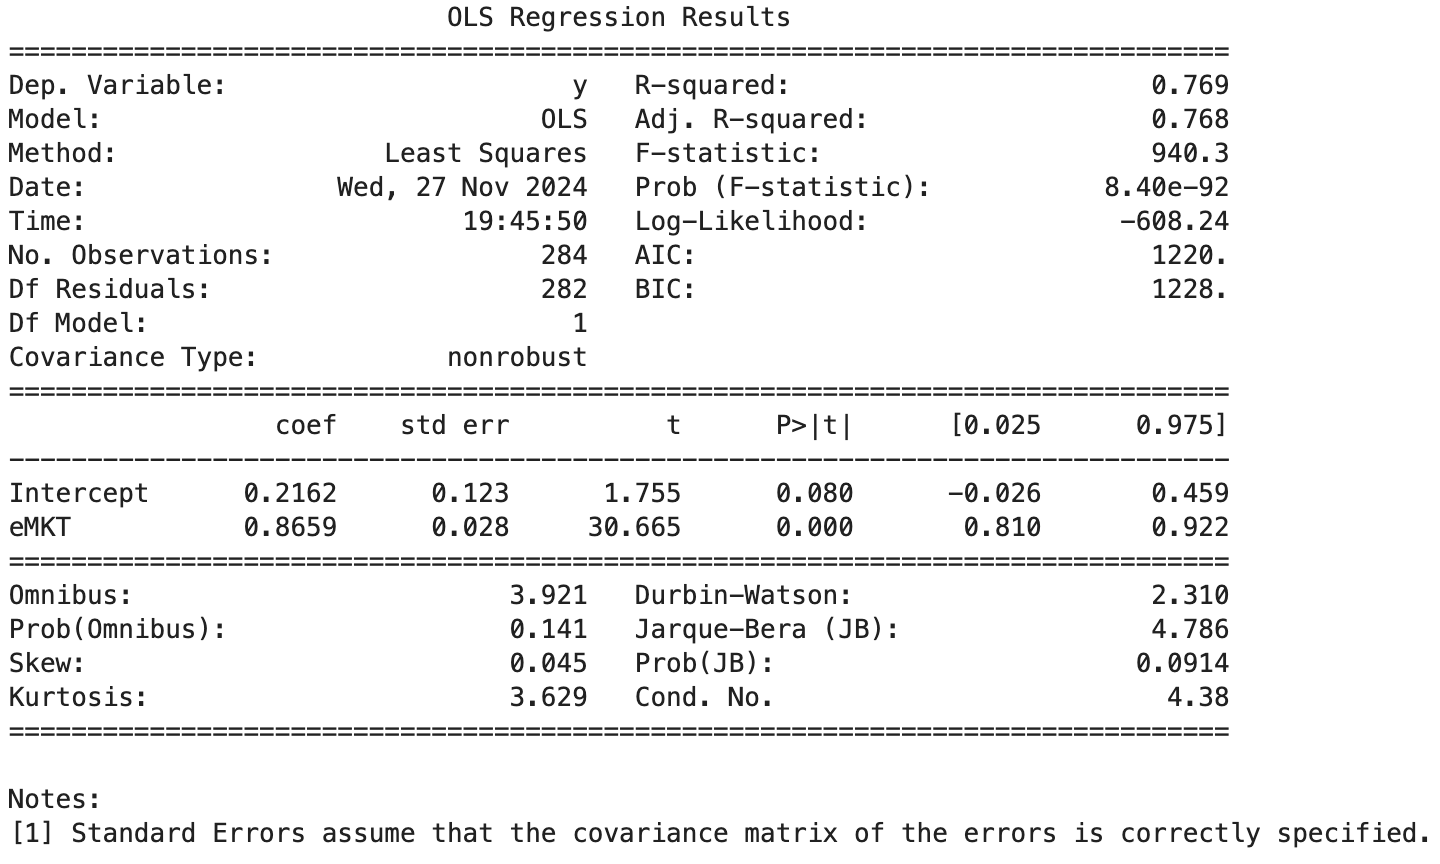
\includegraphics[width=0.8\textwidth]{images/7_4.png}
    \caption{Regression summary for ePortfolio.}\label{fig:7_4}
\end{figure}

\textbf{Beta and Alpha:}
\begin{itemize}
    \item Beta: The beta for eMKT decreased from 0.8659 in the single-factor model to 0.7892 in the multivariate model,
    reflecting the inclusion of additional explanatory factors.
    \item Alpha: Both models produced insignificant alphas, with a decrease from 0.2162 (single-factor model) to 0.1628
    (multivariate model).

\end{itemize}

\subsection{Residual Analysis:}
We examined the residuals of both models to assess their behavior over time and distributional properties.

\textbf{Residual Variance:} CAPM Residuals displayed greater variance (blue line in Figure~\ref{fig:7_5}), consistent with a
poorer fit, while Multivariate Model Residuals' variance was lower (red line in Figure~\ref{fig:7_5}), indicating a better fit.

\begin{figure}[h!]
    \centering
    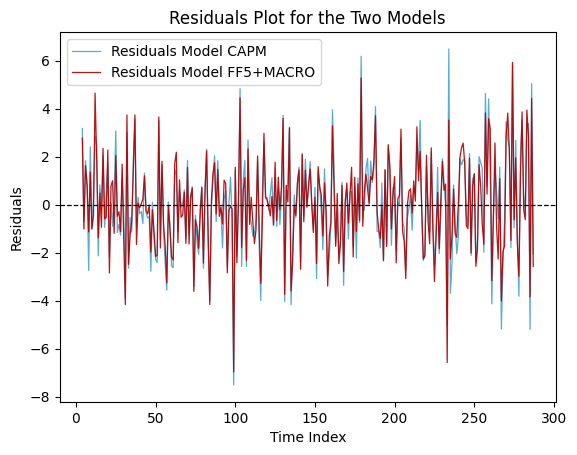
\includegraphics[width=0.8\textwidth]{images/7_5.png}
    \caption{Residals of CAPM against the model built with FF5  and MACRO.}\label{fig:7_5}
\end{figure}

\textbf{Residual Distribution:} CAPM Residuals followed a normal distribution but with a longer left tail, suggesting the
presence of outliers (Figure~\ref{fig:7_6}).

\begin{figure}[h!]
    \centering
    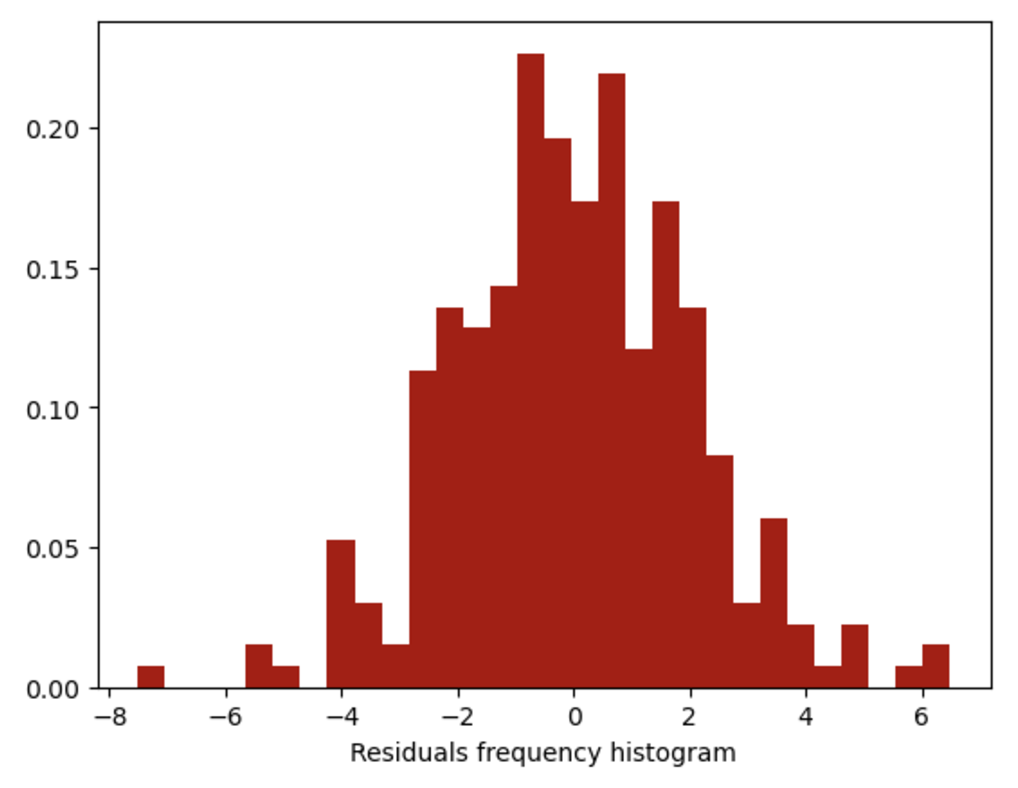
\includegraphics[width=0.8\textwidth]{images/7_6.png}
    \caption{Histogram of residuals for univariate model.}\label{fig:7_6}
\end{figure}

Multivariate Model Residuals also followed a normal distribution but were more concentrated around the mean 
(Figure~\ref{fig:7_7}), reflecting the better explanatory power of the model.

\begin{figure}[h!]
    \centering
    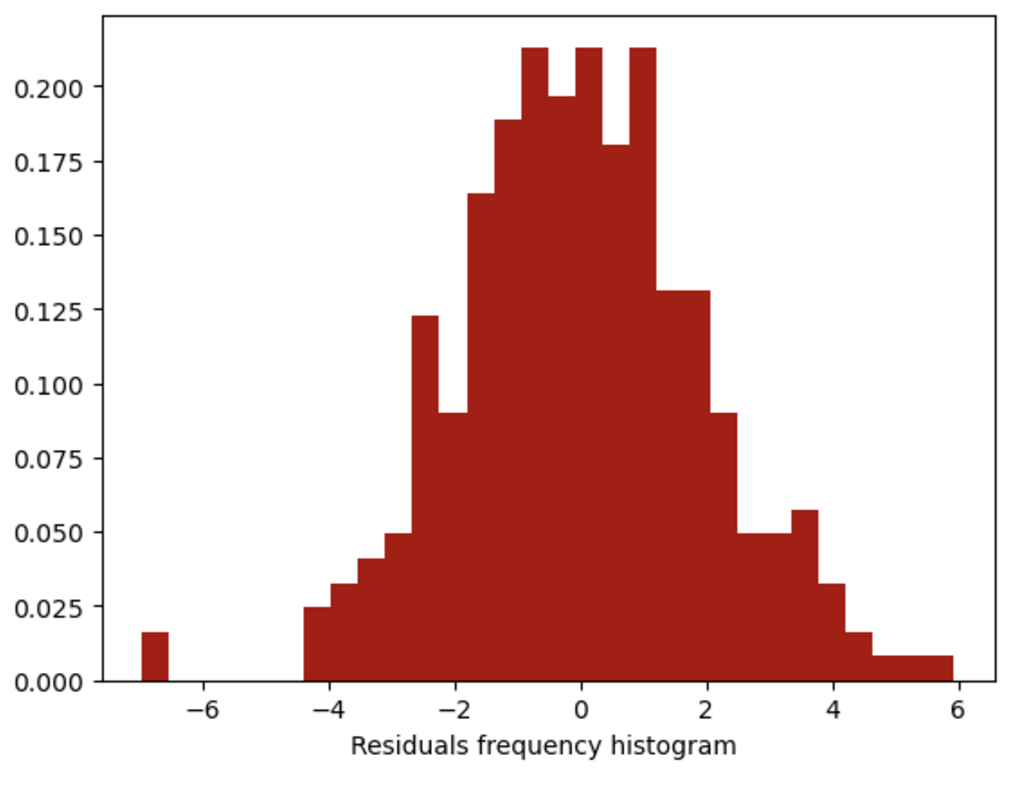
\includegraphics[width=0.8\textwidth]{images/7_7.png}
    \caption{Histogram of residuals for multivariate model.}\label{fig:7_7}
\end{figure}

\textbf{Residual Correlation:} As shown in Figure~\ref{fig:7_8}, residuals from both models had low autocorrelation, 
indicating reliable coefficient estimation.

\begin{figure}[h!]
    \centering
    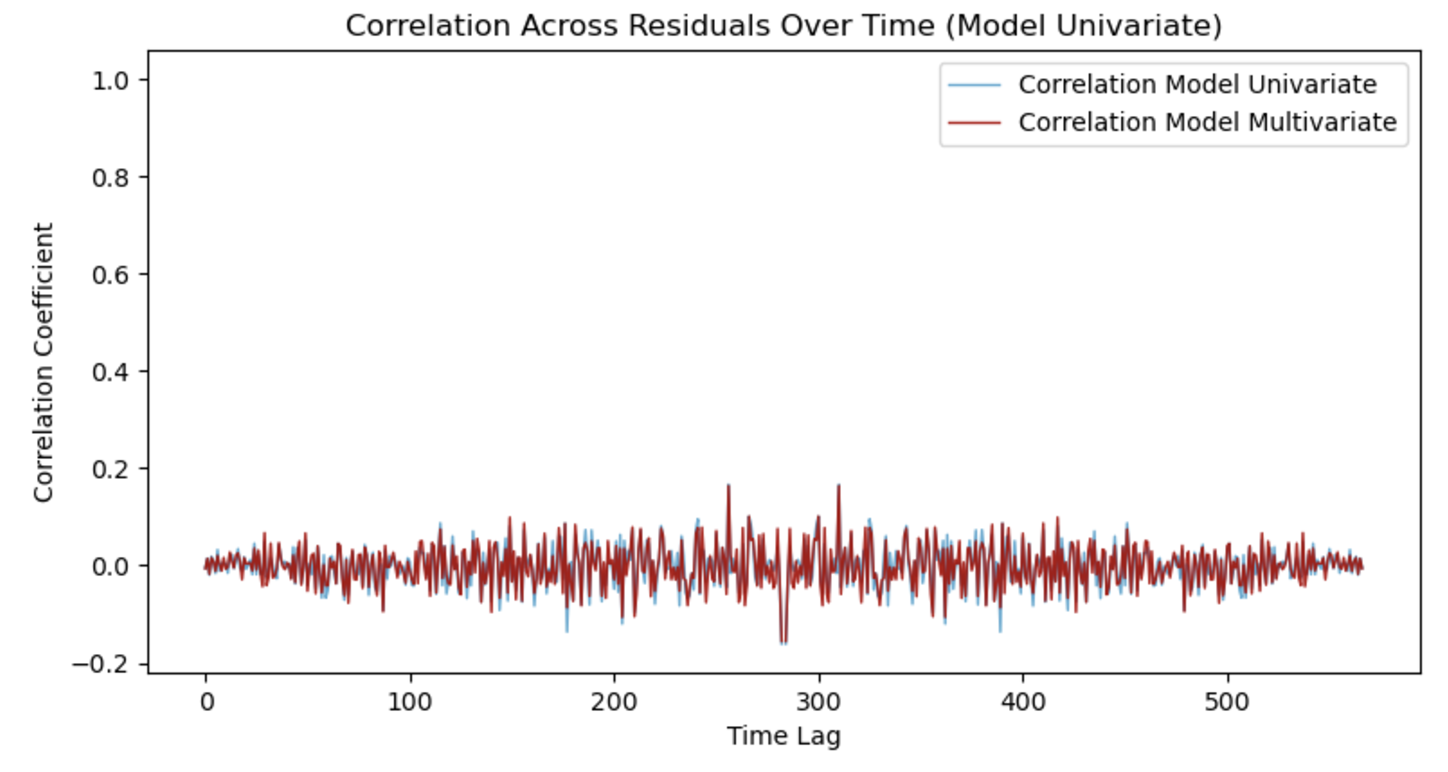
\includegraphics[width=0.8\textwidth]{images/7_8.png}
    \caption{Correlation of residuals over time.}\label{fig:7_8}
\end{figure}


\subsection*{Conclusion}
By incorporating the Fama-French factors and additional macroeconomic variables into the CAPM framework, we achieved a model
with improved explanatory power.
The multivariate model captures sector dynamics more effectively than the single-factor CAPM, as evidenced by better residual 
behavior and higher adjusted $R^2$.



